\section{稀疏图作为预条件}
\label{sec:graph-sparse-preconditioning}

拿到一张谱近似图之后，一个直接的用途是帮助求解原图上的拉普拉斯方程$\bm L_G\bm x=\bm b$。

求解的基本循环是这样的。给定当前的猜测$\bm x$，先算出它在原图上还差多少——残差$\bm r=\bm b-\bm L_G\bm x$。如果能精确解一次$\bm L_G\bm z=\bm r$，那么把$\bm z$加到$\bm x$上就直接补齐了差额。但这需要再解一次原图方程，和原问题一样难。

换一个思路：用边数少得多的近似图$\mathcal H$来求方向。也就是解$\bm L_H\bm z=\bm r$，把$\bm z$作为修正方向。这个方向不完全正确，因为$\bm L_H$和$\bm L_G$不一样。但如果两者足够接近，方向偏差不大，沿着它调整后再回到原图检查残差，几轮下来就能逼近真解。每轮用原图算残差确保终点准确，用稀疏图算方向减少计算量——这就是预条件的思路。

设原图$\mathcal G$连通，相容右端$\bm b\in\bm 1^\perp$，取$\mathcal G$的一个$\varepsilon$谱近似图$\mathcal H$（$0<\varepsilon<1$），以其拉普拉斯矩阵$\bm M=\bm L_H$作为预条件矩阵。在正交补空间$\bm 1^\perp$上，$\bm L_G$与$\bm M$均对称正定。下面的定理给出预条件算子的条件数上界以及\term{预条件共轭梯度法}（preconditioned conjugate gradient method，PCG）的收敛速度。

\begin{theorem}[谱近似预条件的条件数与收敛界]
\label{prop:graph-sparse-preconditioner}
设连通图$\mathcal G$的替代图$\mathcal H$满足$(1-\varepsilon)\bm L_G\preceq\bm M=\bm L_H\preceq(1+\varepsilon)\bm L_G$（$0<\varepsilon<1$）。在$\bm 1^\perp$上定义对称正定预条件算子$\bm A=\bm M^{-1/2}\bm L_G\bm M^{-1/2}$，则：
\begin{enumerate}
  \item 广义Rayleigh商与预条件算子$\bm A$的谱条件数满足
  \begin{equation}
  \frac{1}{1+\varepsilon}
  \leq
  \frac{\bm x^\top\bm L_G\bm x}{\bm x^\top\bm M\bm x}
  \leq
  \frac{1}{1-\varepsilon}\quad(\forall\bm x\in\bm 1^\perp\setminus\{\bm 0\}),
  \qquad
  \kappa_2(\bm A)\leq\frac{1+\varepsilon}{1-\varepsilon}.
  \label{eq:graph-sparse-preconditioned-condition}
  \end{equation}
  \item 以$\bm M$为预条件矩阵求解$\bm L_G\bm x=\bm b$（$\bm b\in\bm 1^\perp$，记零均值精确解为$\bm x_*=\bm L_G^\dagger\bm b$），预条件共轭梯度法第$k$步迭代解$\bm x^{(k)}$满足
  \begin{equation}
  \lVert\bm x^{(k)}-\bm x_*\rVert_{\bm L_G}
  \leq
  2\left(\frac{\sqrt\kappa-1}{\sqrt\kappa+1}\right)^k
  \lVert\bm x^{(0)}-\bm x_*\rVert_{\bm L_G},
  \qquad \kappa=\kappa_2(\bm A)\leq\frac{1+\varepsilon}{1-\varepsilon}.
  \label{eq:graph-sparse-preconditioned-cg-error}
  \end{equation}
\end{enumerate}
\end{theorem}

\begin{proof}
（1）对任意非零$\bm x\in\bm 1^\perp$，将$(1-\varepsilon)\bm x^\top\bm L_G\bm x\leq\bm x^\top\bm M\bm x\leq(1+\varepsilon)\bm x^\top\bm L_G\bm x$移项取倒数，即得广义Rayleigh商夹逼式：
\begin{equation}
\frac{1}{1+\varepsilon}
\leq
\frac{\bm x^\top\bm L_G\bm x}{\bm x^\top\bm M\bm x}
\leq
\frac{1}{1-\varepsilon}.
\label{eq:graph-sparse-preconditioned-rayleigh}
\end{equation}
作可逆坐标变换$\bm y=\bm M^{1/2}\bm x\in\bm 1^\perp$，则$\frac{\bm x^\top\bm L_G\bm x}{\bm x^\top\bm M\bm x}=\frac{\bm y^\top\bm A\bm y}{\bm y^\top\bm y}$正是$\bm A=\bm M^{-1/2}\bm L_G\bm M^{-1/2}$的普通Rayleigh商。因此$\lambda_{\min}(\bm A)\geq\frac{1}{1+\varepsilon}$且$\lambda_{\max}(\bm A)\leq\frac{1}{1-\varepsilon}$，两者相除即得$\kappa_2(\bm A)=\frac{\lambda_{\max}(\bm A)}{\lambda_{\min}(\bm A)}\leq\frac{1+\varepsilon}{1-\varepsilon}$。

（2）将$\bm x=\bm M^{-1/2}\bm y$代入$\bm L_G\bm x=\bm b$并左乘$\bm M^{-1/2}$，转化为等价的对称正定系统$\bm A\bm y=\bm M^{-1/2}\bm b$（精确解为$\bm y_*=\bm M^{1/2}\bm x_*$）。对任意向量$\bm e=\bm x-\bm x_*$，对应变换后误差$\bm d=\bm y-\bm y_*=\bm M^{1/2}\bm e$的$\bm A$-能量范数平方恰好等于$\bm e$的原图$\bm L_G$-能量范数平方：
\[
  \lVert\bm d\rVert_{\bm A}^2=\bm d^\top\bm A\bm d=(\bm M^{1/2}\bm e)^\top\bm M^{-1/2}\bm L_G\bm M^{-1/2}(\bm M^{1/2}\bm e)=\bm e^\top\bm L_G\bm e=\lVert\bm e\rVert_{\bm L_G}^2.
\]
直接对$\bm A\bm y=\bm M^{-1/2}\bm b$应用第~\ref{sec:electrical-numerical-solve}小节的共轭梯度误差界~\eqref{eq:electrical-cg-error}，即得式~\eqref{eq:graph-sparse-preconditioned-cg-error}。
\end{proof}

在实际执行预条件共轭梯度法时，无需显式计算平方根$\bm M^{1/2}$，而是在原坐标下每轮只做两项核心操作：先在原图$\mathcal G$上计算一次矩阵向量乘法$\bm L_G\bm p$以更新步长与残差$\bm r$，再在稀疏图$\mathcal H$上求解一次预条件方程$\bm M\bm z=\bm r$以获得修正方向$\bm z$（完整算法递推见\BookChapterRef{chap:krylov-methods}{卷二“Krylov子空间法”章}）。

若采用单点接地方式，只需在$\mathcal G$和$\mathcal H$中选取同一个接地点$q$：将接地点坐标取零的向量代入式~\eqref{eq:graph-spectral-approximation-energy}，即知两个$(n-1)\times(n-1)$约化正定矩阵$\overline{\bm L}_G$与$\overline{\bm M}=\overline{\bm L}_H$满足完全相同的谱近似界和条件数上界~\eqref{eq:graph-sparse-preconditioned-condition}。

\paragraph{一个完整的迭代例子}

用四点五边图直接看预条件后的效果。令$\mathcal G$为单位权五边图，$\mathcal H$删去对角线$13$后只保留单位权四环。两图在$\bm 1^\perp$上有三个独立的零和方向。

先看$\bm u=(1,0,-1,0)^\top$。对角边两端之差为$2$，贡献能量$4$，加上四条环边各$1$，原图能量为$8$。四环没有对角边，能量只有$4$。广义Rayleigh商$8/4=2$。

再看与$\bm u$正交的零和方向，比如$\bm v=(0,1,0,-1)^\top$。此时对角边两端同值$0$，不贡献能量。两图能量都是$4$（该向量长度平方为$2$、特征值为$2$），商为$1$。

还有一个方向（如$(1,-1,1,-1)^\top/2$归一化），也可核对对角边上差为零。因此四环$\bm M$在$\bm u$方向的特征值是$2$，添对角边后$\bm L_G$在同方向变为$4$，而其余两个方向上两图一样。预条件矩阵$\bm A$的三个特征值为$1,1,2$。通用界$\varepsilon=1/2$给出条件数上界$(1+1/2)/(1-1/2)=3$，覆盖了实际条件数$2$。

用同一例子走一轮迭代。设右端$\bm b=\bm u+\bm v$，初值为零。第一次残差就是$\bm b$。在四环上解$\bm M\bm z=\bm b$，得到$\bm z=(\bm u+\bm v)/2$。

沿$\bm z$更新时，步长由原图决定。因为$\bm u,\bm v$正交且长度平方都是$2$，
\[
\bm b^\top\bm z=2,
\qquad
\bm z^\top\bm L_G\bm z=3.
\]
步长为$2/3$。更新后$\bm x^{(1)}=(\bm u+\bm v)/3$。残差为
\[
\bm b-\bm L_G\bm x^{(1)}
=\frac{-\bm u+\bm v}{3}.
\]
这个残差还含两个方向，下一轮用它继续修正。图~\ref{fig:sparsification-preconditioner-step}把两张图的分工画了出来：四环给出修正方向，原图决定步长和检验残差。

\begin{BookInlineFigure}
  \centering
  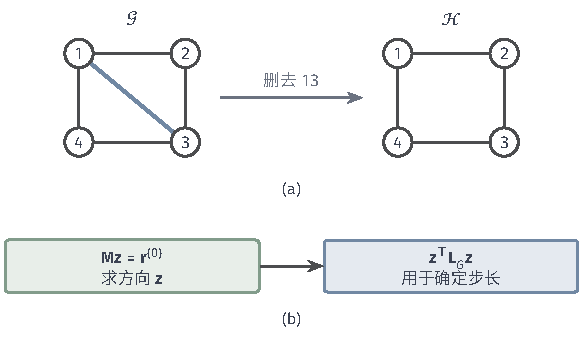
\includegraphics{figures/03-graphs/05-matrices-and-spectra/tikz/sparsification-preconditioner-step/figure.pdf}
  \caption{四点五边图的预条件迭代。（a）原图$\mathcal G$和删去对角边后的四环$\mathcal H$。（b）第一轮用$\mathcal H$的拉普拉斯求方向，用$\mathcal G$的拉普拉斯计算步长和残差。}
  \label{fig:sparsification-preconditioner-step}
\end{BookInlineFigure}

\paragraph{实际代价}

总代价包含三部分：构造稀疏图并准备它的求解器（一次性），每轮在原图上做一次矩阵乘向量（$O(m+n)$），以及每轮在稀疏图上解方程。同一图有多个右端时，可以共享近似图及其分解，把准备成本分摊给多次求解。

稀疏图虽然边少，但直接分解时仍可能产生填充——是否值得要同时比较每轮代价和所需迭代次数。若每轮在近似图上只做有限次内迭代而非精确求解，需要另行控制求解误差，不能直接套用式~\eqref{eq:graph-sparse-preconditioned-cg-error}中精确预条件的结论。
